Historians sometimes gather and analyze mentions of specific query words in archives (Section \ref{s:intro}).
However, much prior work from the HCI, Visualization, and NLP communities focuses on helping people gain high-level overviews of large bodies of text.
We review this overview-oriented literature in Section \ref{s:related_work_overview}.
In Section \ref{s:related_work_search}, we also review another literature on search-based systems, which focus on retrieving text from a corpus in response to a user query.
This search-based approach seems better suited to mention gathering and analysis, as search-based systems can help historians find and review query mentions in a corpus.
Much evidence (Section \ref{s:intro} and Table \ref{t:baselines}) also suggests that search-based systems are central to contemporary historical practice.

In presenting prior work, we emphasize common user interface design patterns \cite{Tidwell}, shared among multiple prior systems.
Interface design patterns are ``concrete bundles of components'' \cite{DesigningInterfaces} that help a user achieve some task. 
We say that \textit{overview design patterns} (Section \ref{s:related_work_overview}) help people survey the contents of archives, and that \textit{search design patterns} (Section \ref{s:related_work_search}) help people query for specific selections from a body of text.
Table \ref{t:baselines} offers a summary of major design patterns from prior work.
Some individual systems (e.g., Expedition \cite{expedition}) may implement both overview and search patterns. Finally, we conclude this Section by discussing \ours~within the context of prior work (Section \ref{s:related_comparison})

\subsection{Overview design patterns}\label{s:related_work_overview}

\subsubsection{\textbf{Word clustering}}\label{s:word_clustering_family}

Because people often can not review every document in a large corpus, many prior text analytics tools such as Termite \cite{termite}, TIARA \cite{tiara}, Overview \cite{overview}, RoseRiver \cite{HierarchicalTopics}, TextFlow \cite{textflow}, Serendip \cite{serendip}, HierarchicalTopics \cite{HierarchicalTopics_Dou}, and ConVisIT \cite{tiisclusterthree} try to suggest overall themes in a body of text by identifying and displaying groups of thematically-related words in a user interface.
We describe this approach as the word clustering design pattern.

Many systems which implement the word clustering pattern are based on prior work from NLP, information retrieval, and text mining, focused on identifying and representing patterns of co-occurring words using methods such as topic models \cite{blei2003latent} and word embeddings \cite{word2vec}.\footnote{The system Themail \cite{themail} clusters words by time, instead of by co-occurrence statistics.
Because this system shows lists of related words (related by time period), we say the system implements word clustering.
Similarly, VisGets shows clusters (of document tags) defined by a user's selection in the interface \cite{visgets}, which we consider to be a form of clustering.}
Researchers in HCI and Visualization extend this work by considering how to present such patterns in a graphical interface;
some systems show changes in cluster patterns across time \cite{tiara,HierarchicalTopics,textflow} (e.g., Figure \ref{f:wordclustering_family}), others do not show time-based topics \cite{termite,overview}. 
Because automatic clusters may not match human mental models of a corpus, one line of work investigates human-in-the-loop techniques, which allow people to modify word clusters through interactions with a GUI \cite{Interactive_Topic_Modeling, tiisclusterone, tiisclustertwo, tiisclusterthree, architext, topiclens, starspire}.

Word clustering has a clear role in historical research.
In query-oriented settings, clustering methods may help people formulate queries they had not considered \cite{Underwood}. 
Moreover, specialized and computationally-oriented digital humanists \cite{poetics_issue} and historians \cite{programminghistorianldatutorial} have used word clusters from topic models for corpus analysis.
Nevertheless, successful application of topic modeling requires specialized knowledge and extensive interpretive effort \cite{Baumer,schmidt2012words}, making this method less accessible to a broader audience of historians.  
Additionally, many historians approach archives looking for mentions of what Allen and Sieczkiewicz describe as ``specific keywords'' \cite{allen} rather than looking to explore word cluster overviews from a topic model API.
Because we design for historians investigating known query terms (Section \ref{s:intro}), we do not employ the word clustering pattern in the \ours~interface.

\subsubsection{\textbf{Textual and visual summaries}}\label{s:textual_summary_family}

Rather than showing lists of related words to offer a corpus overview, a large body of work on text summarization from NLP \cite{das2007survey} instead attempts to create short paragraphs which convey the most ``important'' information in a corpus, by selecting a collection of sentences or sentence fragments from input documents to form an output summary.
(This is sometimes described as extractive summarization \cite{das2007survey} because the output text is extracted from input text.) 
User-facing systems such as Newsblaster \cite{NewsblasterMain} and NSTM \cite{bambrick-etal-2020-nstm} apply this research by showing such textual summaries in a graphical interface.
We say that such tools implement the textual summary design pattern (Figure \ref{f:textual_summary_family}). 
Other closely related work from text visualization considers how to present summary text in specialized visual layouts such as Document Cards \cite{DocumentCards}, Phrase Nets \cite{phrasenet}, or Word Trees \cite{wordtree}.
We say that these interfaces offer structured visual summaries, as they place summary text within some structured visual format (e.g., a directed graph \cite{phrasenet}).

Like word clusters, both traditional text summaries and structured visual summaries do not seem to help with mention gathering and analysis. A user can't turn to these forms of summaries to find and review query mentions because ``important'' sentences selected for inclusion in summary output may or may not contain a given query word.
Moreover, traditional approaches typically do not explain \textit{how} ``important'' information is chosen, which may be important in the history domain (Section \ref{s:discussion_NLP}).

However, two ideas from the text summarization literature may help historians perform mention gathering and analysis.
First, work in query-focused summarization tries to identify the most salient information in a corpus, based on a user's query \cite{nenkova2012survey}.
Historians might use such query-focused summaries to review keywords in text. 
Query-focused summaries which define \textit{all} query mentions as important enough to warrant inclusion in summary output may be especially helpful (see Section \ref{s:needs_comprehensive}). 
Second, work on sentence compression \cite{Knight2000StatisticsBasedS,filippova-strube-2008-dependency,filippova2015sentence} tries to shorten individual sentences by removing words, usually for the purpose of including more (shortened) sentences in a fixed-length summary. 
These methods, or closely-related sentence fusion techniques \cite{barzilay-mckeown-2005-sentence}, might be used to shorten passages containing query terms to help people quickly review many mentions of a query in context.
We apply these two ideas from text summarization in \ours~(see Section \ref{s:feed_and_viewer} and \ref{s:simplification}).


\begin{figure}[t!]
\captionsetup[subfigure]{}

\begin{tabular}{@{}c@{}}

\begin{subfigure}{\leftwidth}
  {\vspace{\titleoffset}{\textbf{\mbox{Overview}} \\ \textbf{\mbox{patterns}} \\ { \small (Sec.\ \ref{s:related_work_overview})}} }
  \label{f:overview}
\end{subfigure}
\begin{subfigure}{\familypicwidthPlus}
  \centering
  % include second image
  \fbox{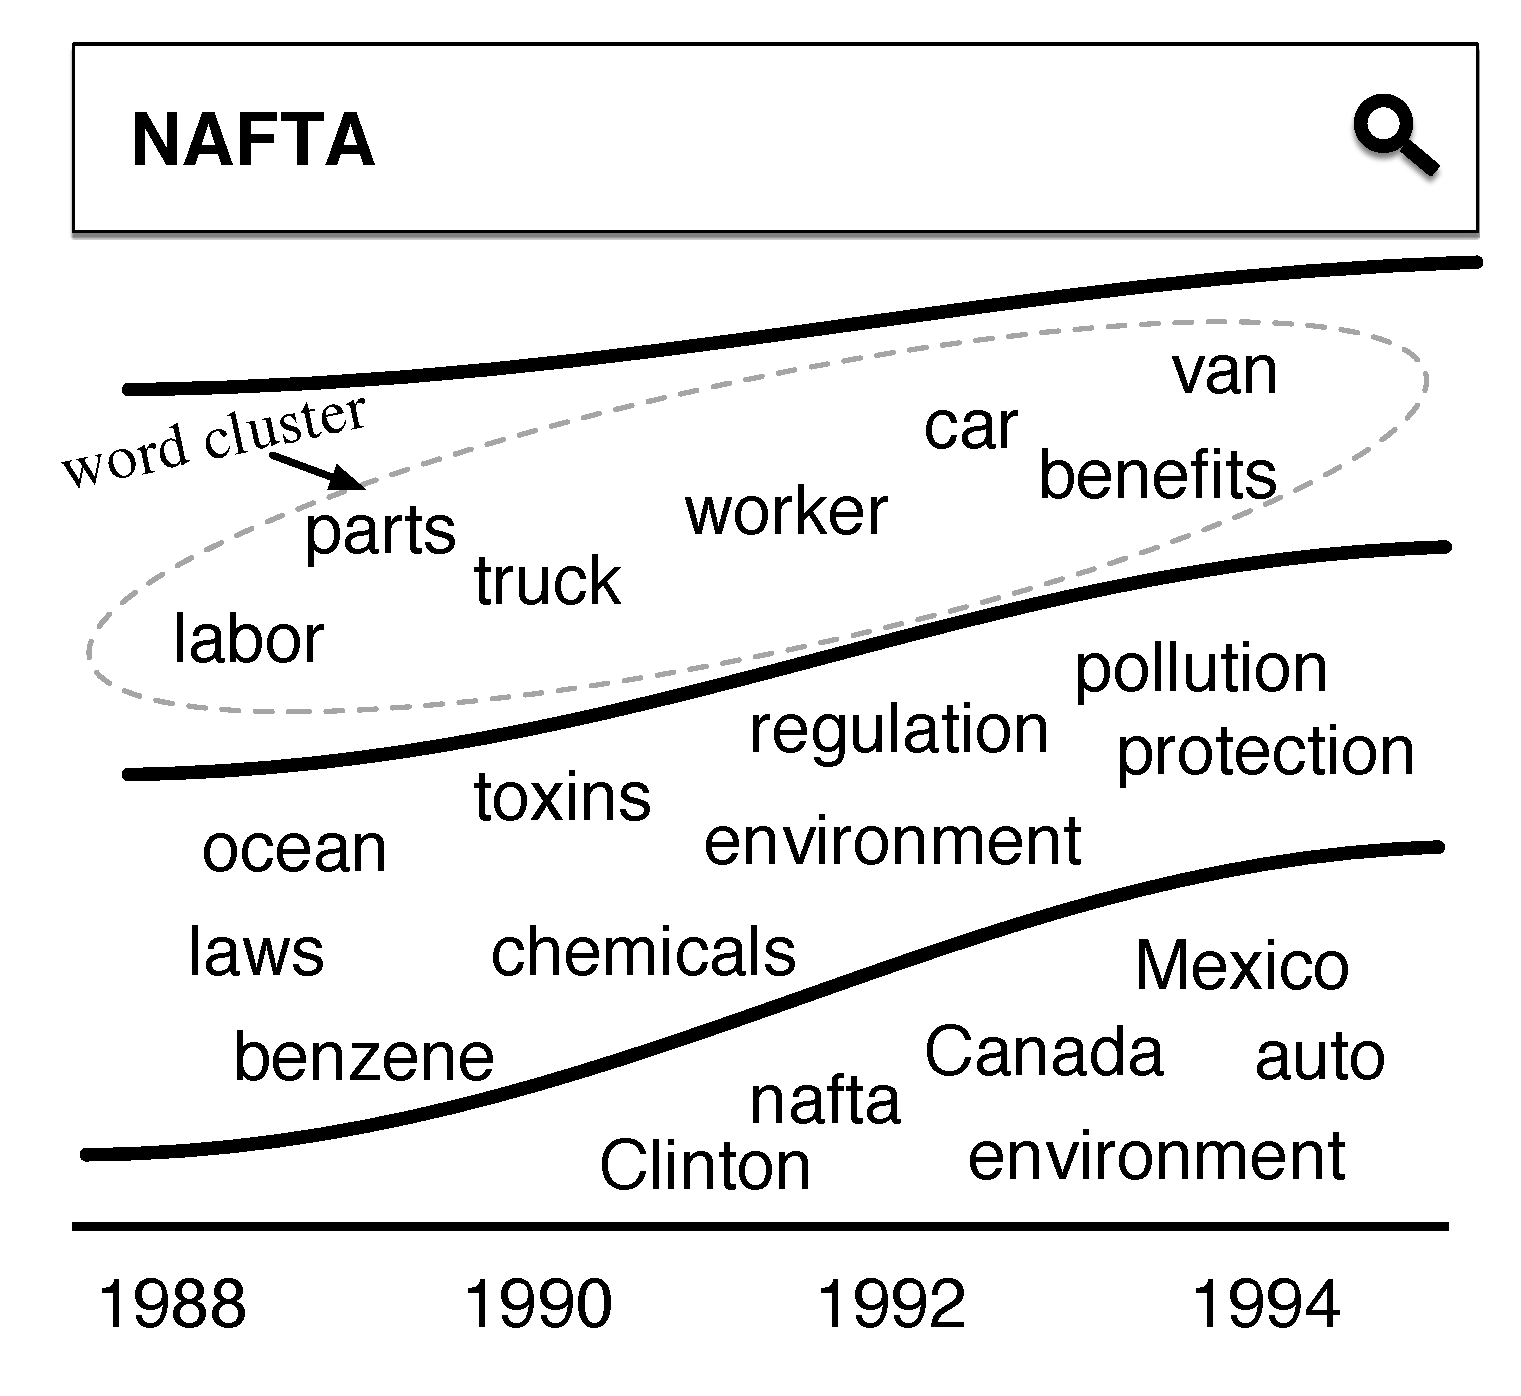
\includegraphics[width=\familypicwidth]{figures/families/clustering.pdf}}
  \caption{\hspace{.4cm}{\small Word clustering (Section \ref{s:word_clustering_family})} \\ \centerline{ \footnotesize Examples: \cite{HierarchicalTopics,overview,termite, tiisclusterone, tiisclustertwo, tiisclusterthree}}  }
  \label{f:wordclustering_family}
\end{subfigure} 
\begin{subfigure}{\familypicwidthPlus}
  \centering
  % include first image \hspace{.35cm} 
  \fbox{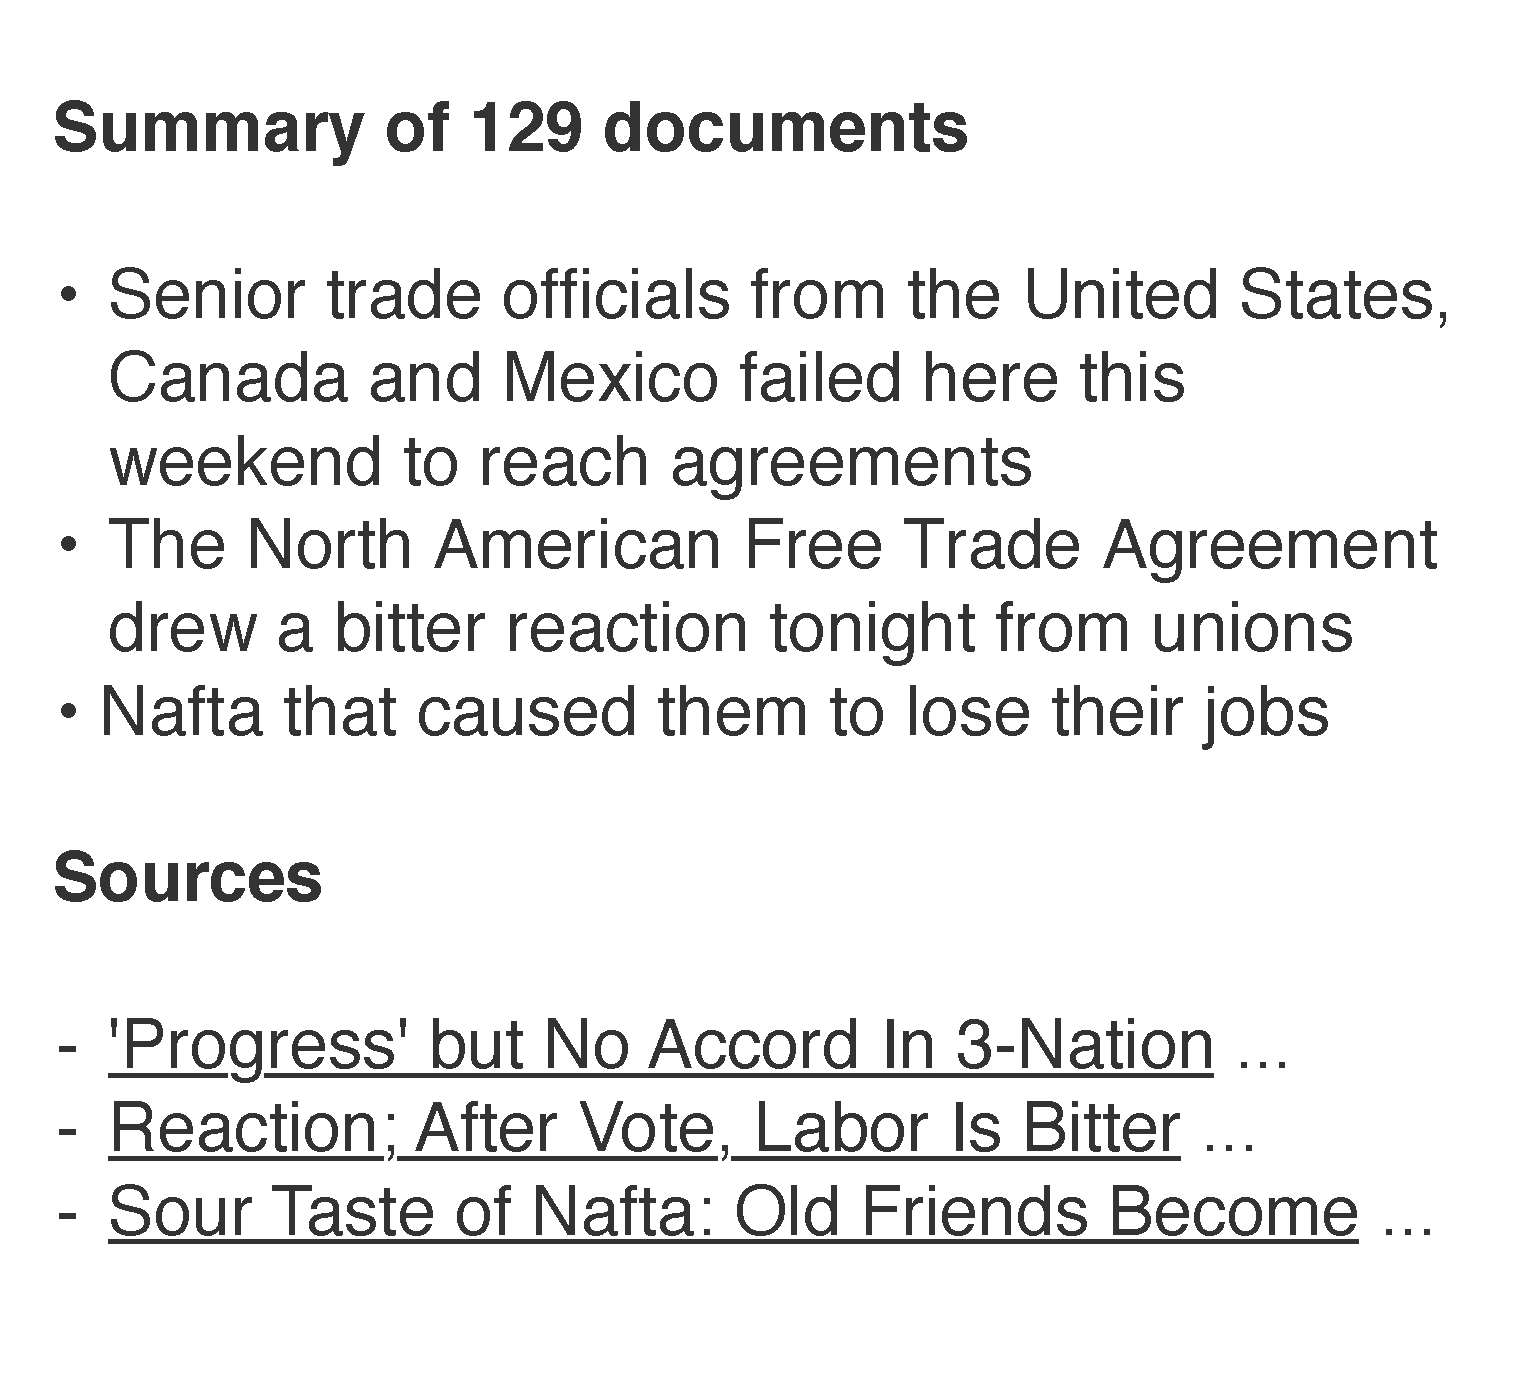
\includegraphics[width=\familypicwidth]{figures/families/summarization.pdf}}\hspace*{-0cm}
  \hspace{.7cm}\caption{\hspace{.0cm} {\small Textual \& visual summary (Sec.\ \ref{s:textual_summary_family})} \\ { \centerline{\footnotesize  \centerline {Examples: \cite{NewsblasterMain, summons, bambrick-etal-2020-nstm} }}}}
  \label{f:textual_summary_family}
\end{subfigure} \\ \\
\begin{subfigure}{1.5cm}
  \textbf{}
\end{subfigure}
%\begin{subfigure}{\familypicwidthPlus}
%  \centering
%  % include first image
%  \fbox{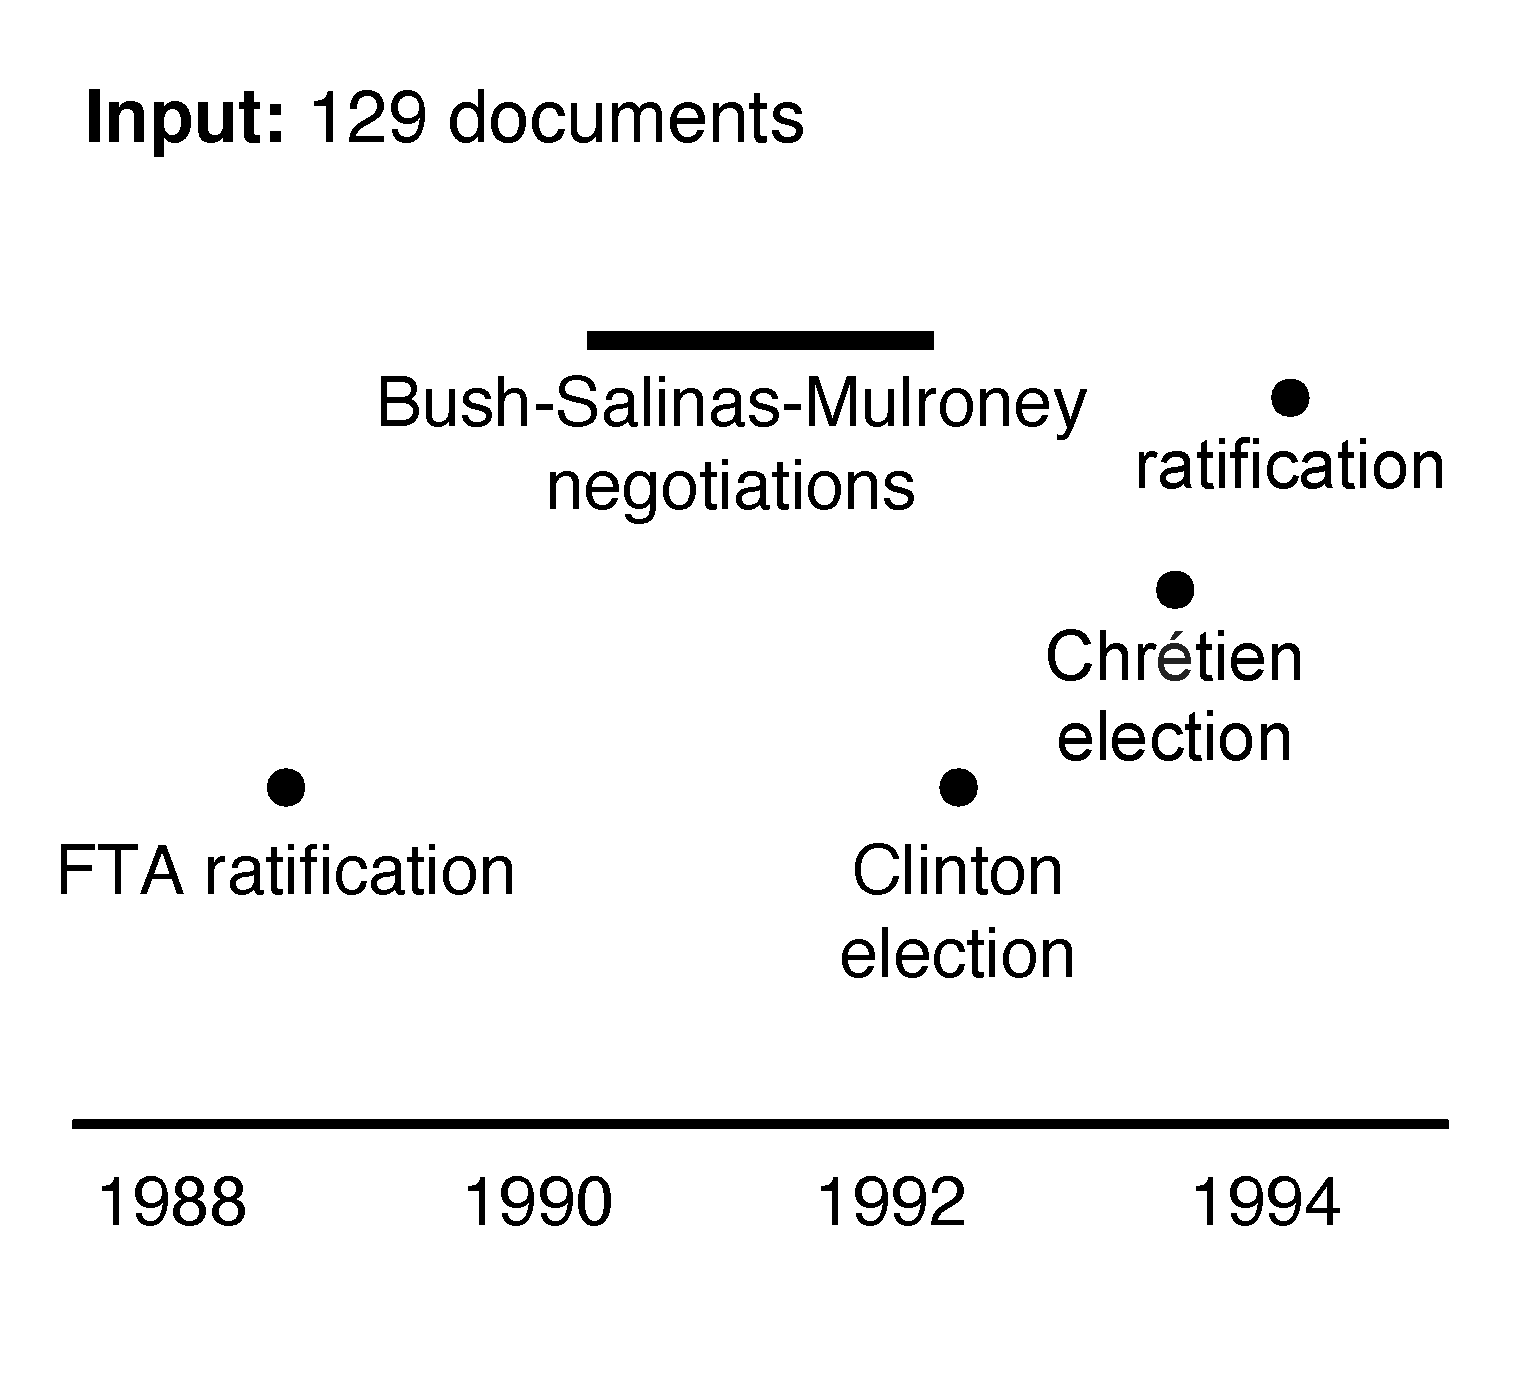
\includegraphics[width=\familypicwidth]{figures/families/timeline.pdf}}
%  \caption{{Visual timeline (Section \ref{s:timeline_family})} \\ 
%  { \centerline{\footnotesize Examples: \cite{LifeLines, TimeLineCurator,james_allan,timelinejs}} }}
%  \label{f:timeline_family}
%\end{subfigure}
\begin{subfigure}{\familypicwidthPlus}
  \centering
  % include second image
  \fbox{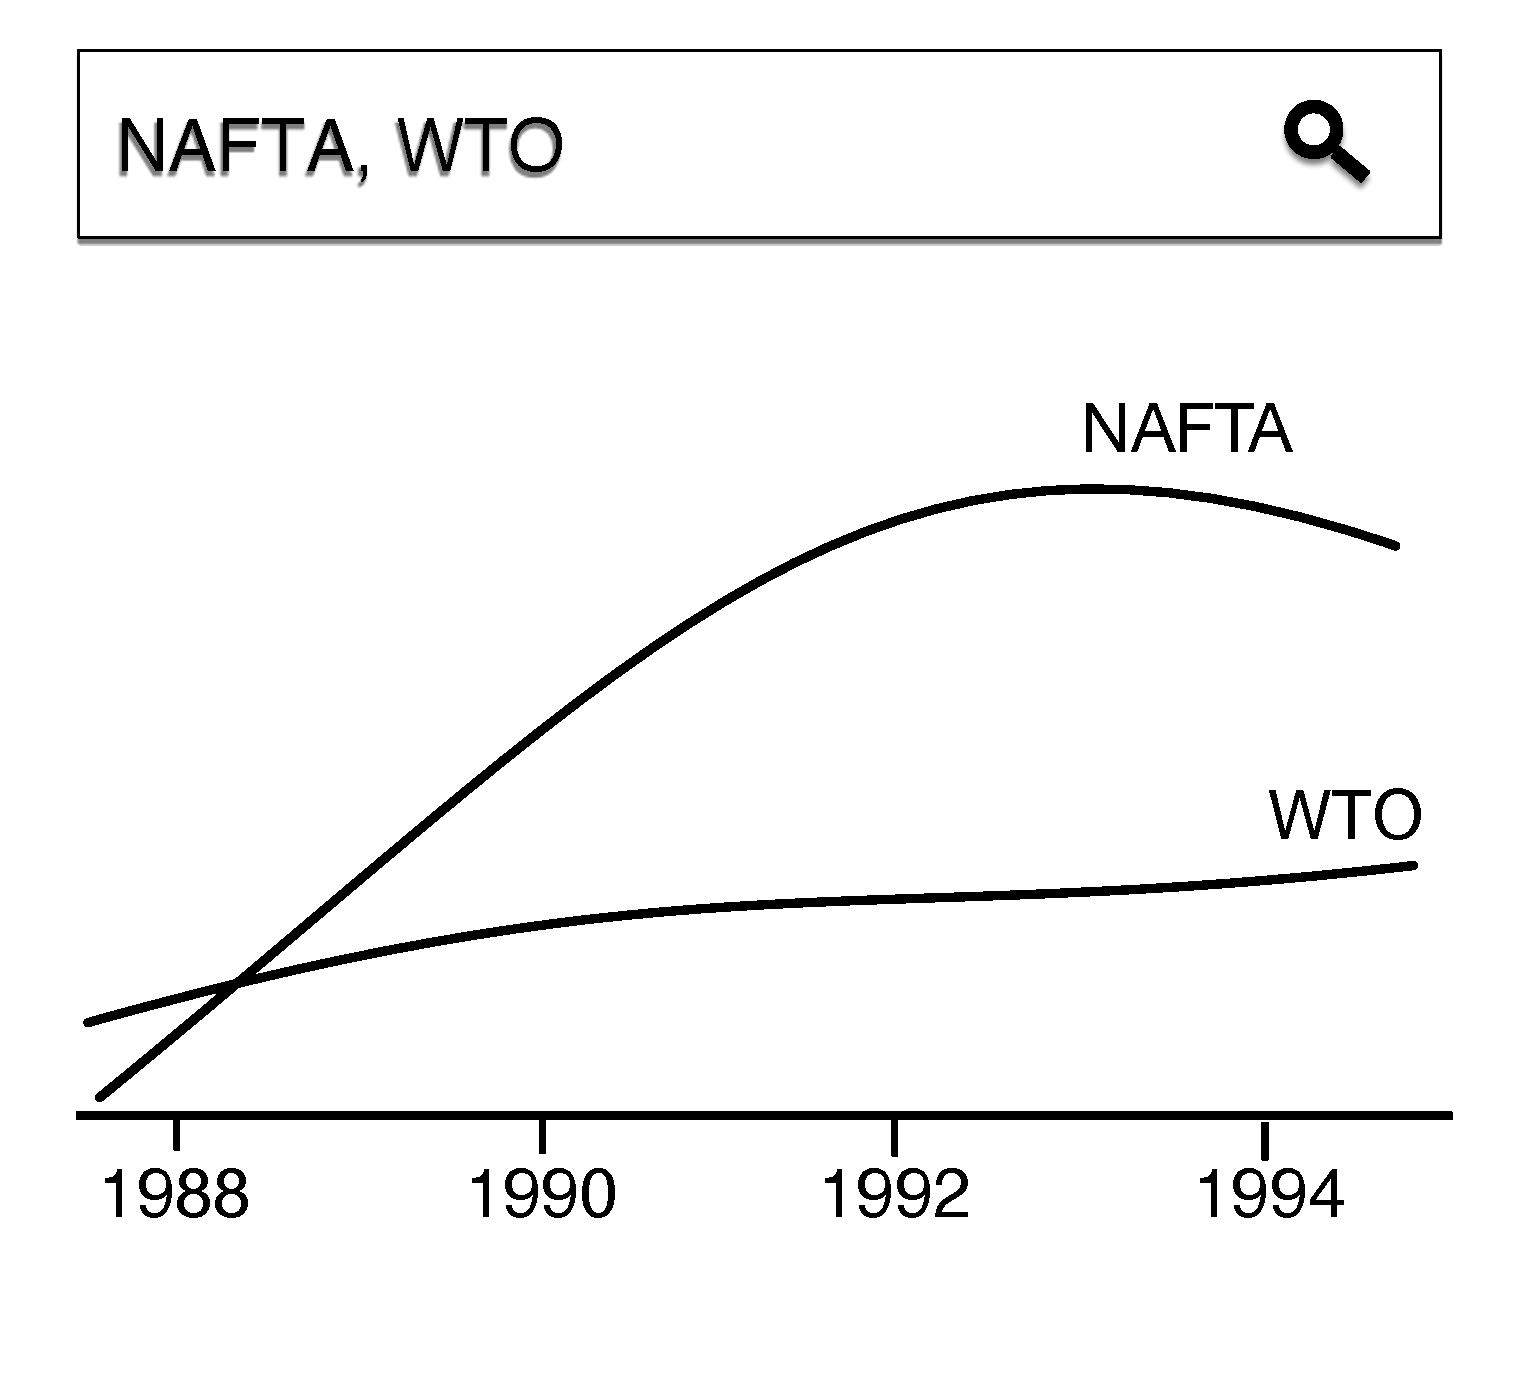
\includegraphics[width=\familypicwidth]{figures/families/timeseries+.pdf}}
  \caption{\hspace{.3cm}{\small Time series plot (Sec.\  \ref{s:time_series_family})} \\ 
  {  \centerline{\footnotesize \hspace{-.4cm} Examples: \cite{ThemeRiver, Michel176, voyant, sotu}}}}
  \label{f:time_series_plus_family}
\end{subfigure} \\ \\    \hline
% % \hspace{-12cm} 
{} \\ 
\begin{subfigure}{\leftwidth}
  {\vspace{\titleoffset}{\textbf{Search} \\  \textbf{patterns}\\ {\small (Sec.\  \ref{s:related_work_search})}}}
\end{subfigure}
\begin{subfigure}{\familypicwidthPlus}
  \centering
  \fbox{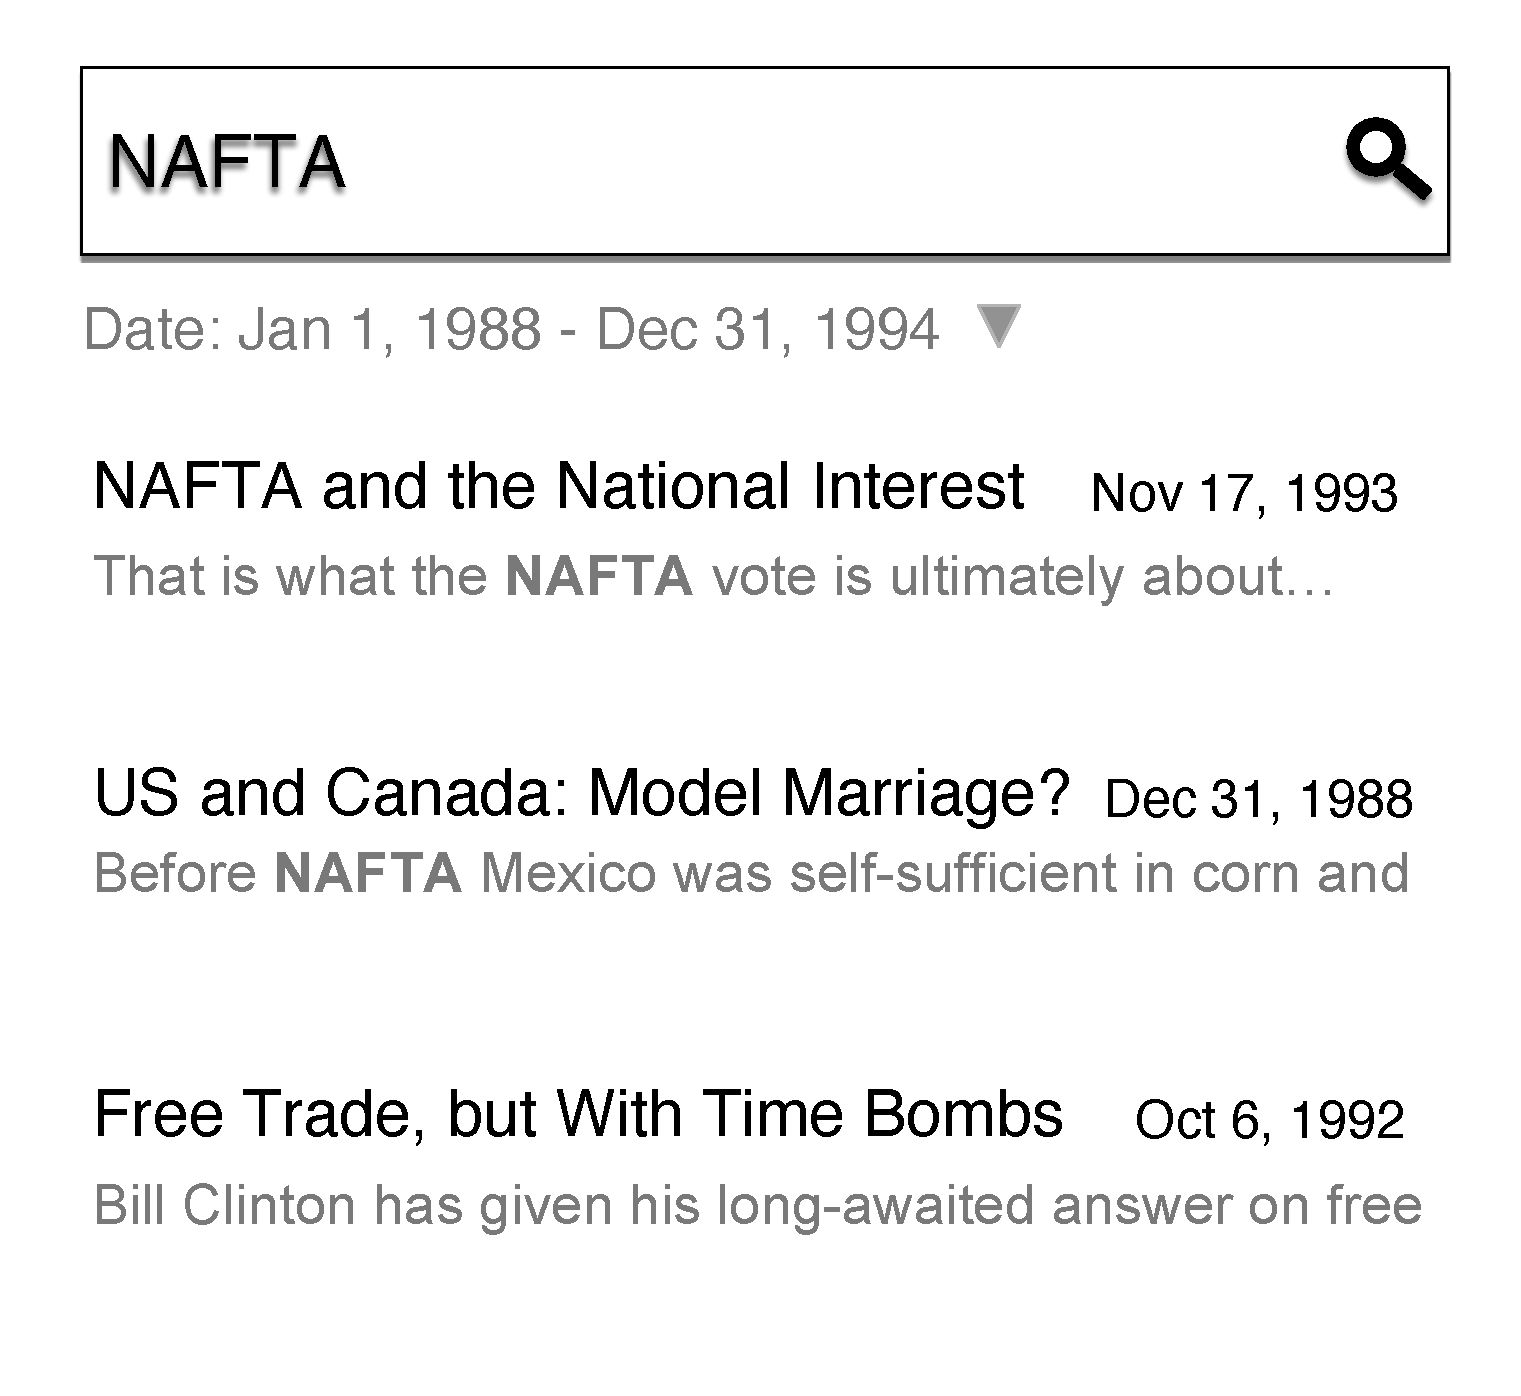
\includegraphics[width=\familypicwidth]{figures/families/search.pdf}}  
  \caption{ {\hspace{.6cm}\small Keyword search (Sec.\  \ref{s:baseline}) } \\ 
   \centerline{\footnotesize Examples: \cite{nytwebsite, TileBars, hotmap, newspapers.com, lucene, voyant}} }
   \label{f:keywordsearch_family}
\end{subfigure}
\begin{subfigure}{\familypicwidthPlus}
  \centering
  \fbox{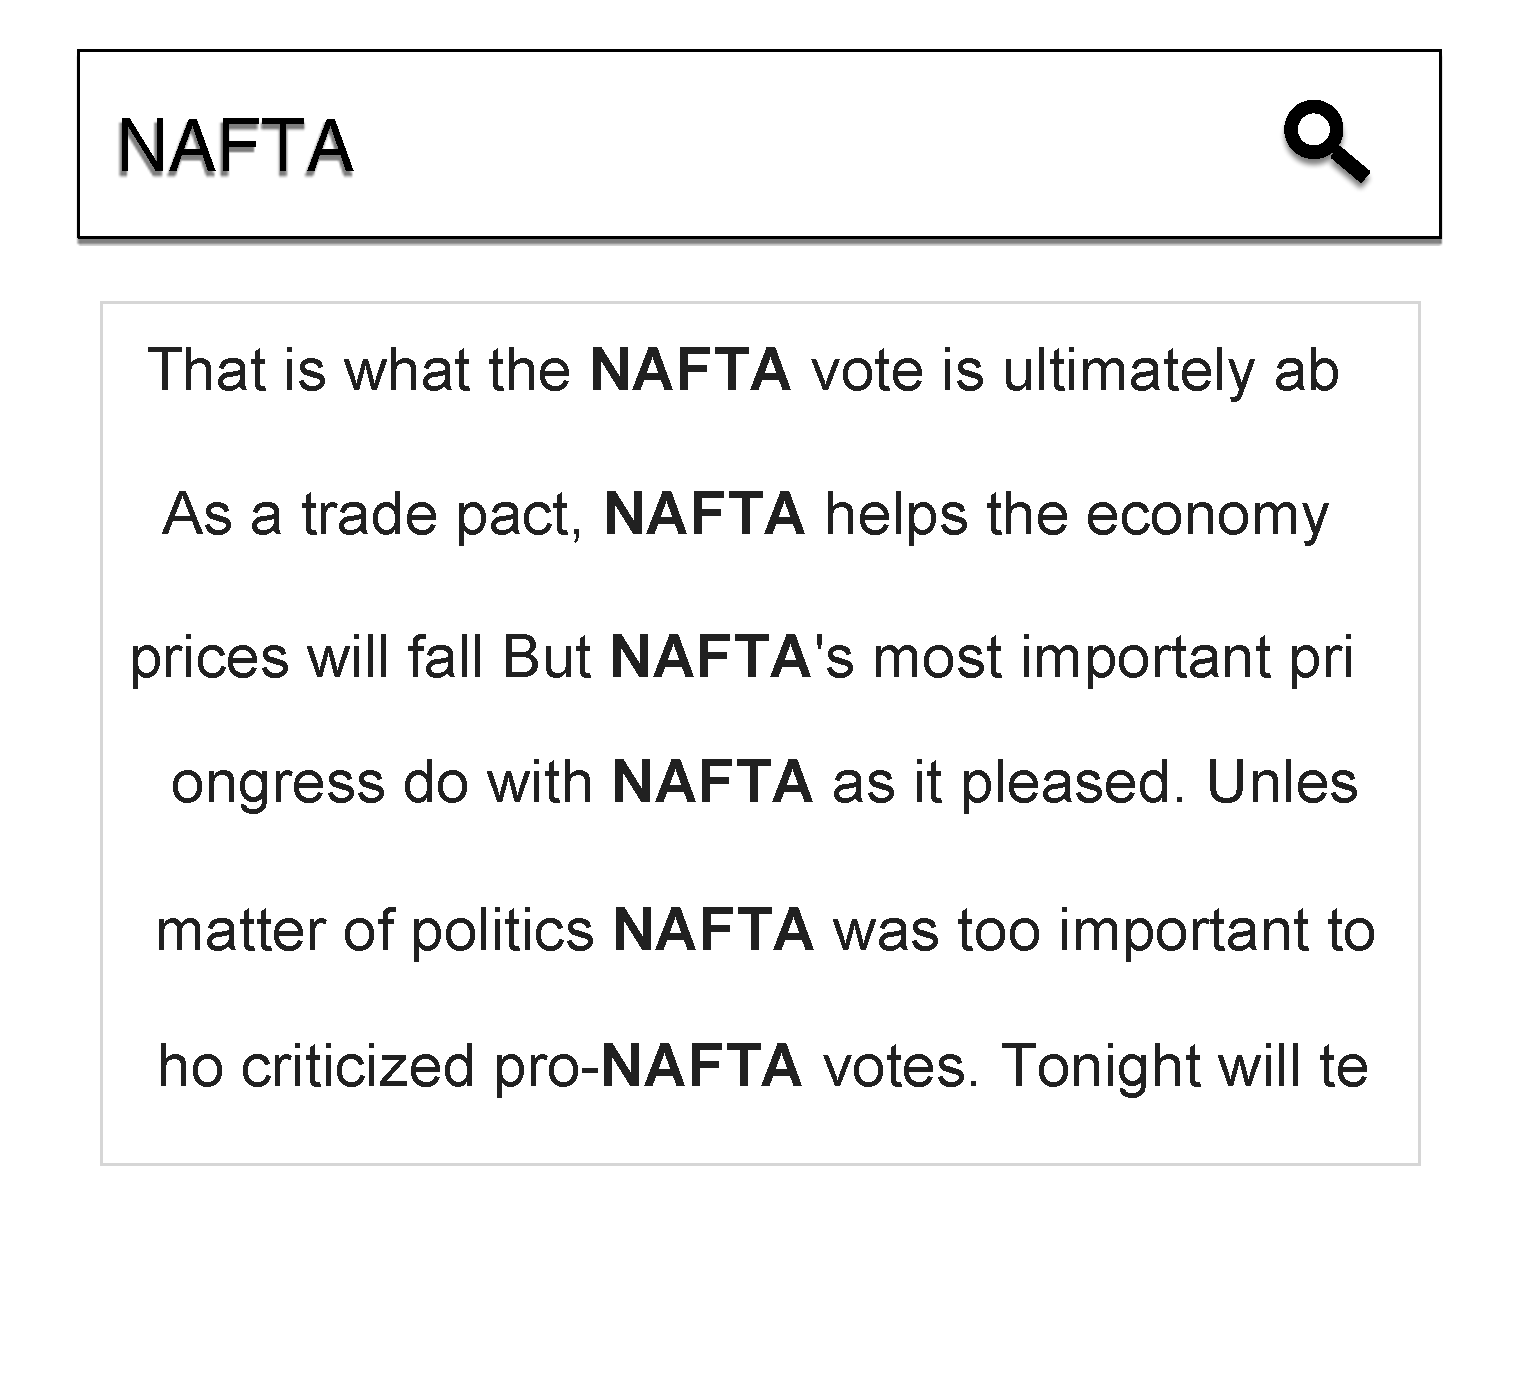
\includegraphics[width=\familypicwidth]{figures/families/kwic2.pdf}}  
  \caption{ {\hspace{.5cm}\small Multi-doc.\ snippet (Sec.\  \ref{s:snippets_family}) } \\ 
  {  \centerline{ \footnotesize Examples:  \cite{Luhn_kwic, oconnor-2014-mitextexplorer, voyant, themail}} }} 
  \label{f:kwic_family}
\end{subfigure} \\ \\ 
\end{tabular}
% push more cites and screenshots to appendix 
% all in one table 
% show what the patterns are clearly and visually consistently 
% adhere to standards in prior work
% 1 X 6 table format (meeting 1/21)
% show all cites 
% ref to sections
% I really like this figure and think it will look terrible w/ heterogenous screenshots
% one page 
% too many cites = line break
% this table holds the most up-to-date version of what systems implement what methods
% \input{samples/tables/family_table}
%\caption{}
\caption[Five major user interface design patterns from prior work]{
\protectWe define five major user interface design patterns from prior work devoted to helping users understand news archives and other corpora (Section \ref{s:related}).
Three of the design patterns focus on helping users gain an overview of archive contents (top two rows).
Two of the design patterns focus on helping the user to search for specific documents or passages from a corpus (bottom row).
Following Tidwell \cite{Tidwell}, this figure presents prototypical wireframes of each design pattern, created by the authors of this work. 
Each example above shows a system presenting results from 129 documents matching the query ``NAFTA'' on a corpus of \textit{New York Times} editorials published between 1988 and 1994. %thesis needs slightly shorter caption for formatting. During thesis compilation families_caption => families_caption_thesis
}\label{f:families_all}
\end{figure}

% http://designinginterfaces.com/firstedition/index.php?page=About_Patterns
% http://www.mit.edu/~jtidwell/common_ground.html => Pointer Shows Affordance


\subsubsection{\textbf{Time series plot}}\label{s:time_series_family}

Instead of showing text to summarize corpus contents, time series plots present the frequency of words or documents across time to offer a visual (rather than textual) corpus overview. 
This pattern is often implemented in text analysis tools \cite{voyant,twitinfo,diamonds,featurelens} and keyword search systems \cite{expedition, TimeExplorer, newspapers.com}.
Some time series visualizations \cite{Michel176, histdiv, TimeExplorer} show the frequency of a single query term across time (e.g., Figure \ref{f:time_series_plus_family}), often using a line chart. 
Others show the frequency of multiple terms (e.g., highest-count words) using a stacked area chart \cite{ThemeRiver,sotu}, and may not require a user-supplied query. 
While time series plots alone can not be used for mention gathering and analysis (because they do not show underlying text from a corpus), 
such visualizations can hint at important events or changes across documents (e.g., Michel et al.\ \cite{Michel176}).
We thus implement this design pattern in \ours~(Section \ref{s:system_ts}).

\subsection{Search design patterns}\label{s:related_work_search}

\subsubsection{\BaselongnameCap~(baseline)}\label{s:baseline}

Traditional \Baselongname~tools return relevance-ranked lists of documents on a search engine results page (SERP) in response to a free-text query \cite{irbook}.
Because historians often use such tools in practice (Section \ref{s:intro}),
we consider these systems to be baselines for mention gathering and analysis.\footnote{
One strand of humanities scholarship critically investigates how widespread adoption of \Baselongname~tools might be distorting traditional humanistic research \cite{Putnam,FrancesMaule,Underwood}.
}

Although \Baselongname~tools are widely used (Table \ref{t:baselines}), these systems have clear downsides for finding and reviewing query mentions.
First, \Baselongname~systems impose unnecessary burdens from reading and context switching. This is  described in detail in Section \ref{s:intro}. 
Additionally, \Baselongname~systems rank documents according to a computational model of relevance.
This may be undesirable for historians because relevance-ranking introduces opaque algorithmic influence over qualitative conclusions (by guiding people towards particular documents).
Section \ref{s:needs} describes the importance of neutral and comprehensive review in historical research.

{
\begin{table}[t!]
\centering
% \small % uncomment for thesis
\begin{tabular}{rccl}
\toprule
                       & {Relevance ranking} & {Filter by Date} & {Known users}    \\ \midrule
{Chronicling America} & \checkmark                     & \checkmark               & \footnotesize{$\ithree,\ifour,\ifive$,$P4,H1$}          \\
{Newspapers.com}         & \checkmark                     & \checkmark               & \footnotesize{$\ione$,$P1,P4,H2$}     \\
{New York Times Search}       & \checkmark                     & \checkmark              &  \footnotesize{$\ithree,\ifour,\ifive$,$P1$,$P5$,$H1,H2$}  \\
{ProQuest}               & \checkmark                     & \checkmark              & \footnotesize{$\ione$ to $\ifive$, $P1,P3,P4,P5,H1,H2$}      \\  \bottomrule  
\end{tabular}
\caption[Examples of baseline keyword document search systems]{Example baseline keyword document search systems, featuring relevance-ranked search engine results pages and filtering by date. Such features are common in many news archive interfaces \cite{suveyhistorialnewsinterfaces}. Tables in the Appendix provide more details on the backgrounds of known users. 
Above, we use \ione~to \ifive~to indicate all interviewees.
}\label{t:baselines}
\end{table}
}


%%%%$H1$,$P3$ and $P4$ say they find newspapers.com hard to access.


Ranking aside, \Baselongname~tools may also shape user perceptions of the contents of the individual documents in an archive, through displaying single-document summaries (also called query-biased snippets \cite{querybiased}) on the search engine results page.\footnote{
Google sometimes shows complex results snippets on the SERP, using proprietary techniques. 
Brin and Page briefly mention the need for such ``Result Summarization'' in their original paper \cite[Section 6.1]{pagerank}.
} 
For example, Figure \ref{f:keywordsearch_family} displays three sample single-document summaries, showing what a computer deems to be the most important information from three different search results.
Such single-document summaries may be inappropriate for historical research, as some historians may be skeptical of opaque models which select ``important'' information for their review (search engines try to include keywords in snippets, but do not try to explain summaries \cite[Section 6.3.1]{croft2010search}).
Prototypes shown in the Appendix describe our own experiences attempting to apply similar document summarization techniques for historians without success.

\subsubsection{Multi-document snippet}\label{s:snippets_family}

Where \Baselongname~systems return links to single documents in response to a user query,
other systems return collections of smaller units like paragraphs, sentences, or character spans, which are often drawn from multiple documents (see Figure \ref{f:kwic_family}).
We observe two different implementations of this multi-document snippet design pattern in interactive text analytics.

First, multi-document snippet features can be used in word clustering systems to help people investigate mentions of particular clustered words in context.
For example, TIARA \cite{tiara} allows analysts to review individual words from a cluster in underlying text.
However, because TIARA is designed for showing broad themes rather than for reviewing query mentions, 
it does not comprehensively show all mentions of a given word in its multi-document snippet.
Instead, TIARA chooses some selection of mentions for display, optimizing for diversity \cite[Section 6]{tiara}.
Such curation may introduce unwanted algorithmic bias (Section \ref{s:needs_trust}), because the system chooses some but not all query mentions for display.

Additionally, other text analysis systems which are not necessarily focused on clustering sometimes include keyword-in-context (KWIC) views \cite{voyant,oconnor-2014-mitextexplorer}, showing each mention of a query word (or a selection of such mentions) on its own line of text amid immediately surrounding tokens or characters (e.g., Figure \ref{f:kwic_family}).
While this form of multi-document snippet can be used for mention gathering and analysis, KWIC views have some limitations for historical research.
First, in many cases, historians need to investigate particular query mentions within the context of full documents (Section \ref{s:needs_context}). 
While KWIC views may include links to underlying sources, jumping from KWIC views to documents requires context switching into new windows or tabs to gather and analyze evidence.
We explain why this is undesirable in Section \ref{s:intro}.
Second, KWIC views always show some number of pixels, characters or words immediately surrounding each query mention.
This may result in awkward-sounding or choppy snippets that do not include the most salient information in source sentences;
evidence suggests that people dislike awkward-sounding snippets \cite{ryenwhitesnippets}.
Finally, KWIC views do not offer a way to keep track of which mentions have been reviewed during analysis, which may be important in historical research (Sections \ref{s:needs_comprehensive} and \ref{s:tracking}).
Noting these shortcomings, it is possible to interpret certain \ours~features (Section \ref{s:feed_and_viewer} and \ref{s:documentviewer}) as a particular form of KWIC view, addressing some of these limitations.

\subsection{Situating \ours~withing the broader literature on visual analytics for text}\label{s:related_comparison}

Researchers have proposed many approaches to interactive text analytics \cite{tiara,overview,Gorg2013JigsawReflections,serendip,HierarchicalTopics,chuangheer,termite,tiisclusterone,tiisclustertwo,tiisclusterthree,starspire,pivotpaths,eventriver,jasim2021communitypulse}. 
Within this broad literature, \ours~is unique because it is designed to help people find and analyze all occurrences of a query word across a corpus (see Section \ref{s:needs_formal_problem}).
Using terminology from Chuang et al., \ours~differs from prior work because its central ``unit of analysis'' \cite{chuangheer} is the query word in context; the system's~``visual encodings,'' ``modeling decisions'' \cite{chuangheer}, and user interactions were all designed to help people quickly and comprehensively review mentions of a query word across an archive.
For instance, \ours~includes a textual summary feature, that presents a synopsis of all occurrences of a query word in a corpus (Section \ref{s:feed_and_viewer}).

Focusing on query words in context is a departure from prior work in text analytics, which emphasizes other latent and observable textual units of analysis, such as topics \cite{tiara}, events \cite{eventriver}, document metadata \cite{pivotpaths}, interrelated entities \cite{Gorg2013JigsawReflections}, or thematic hierarchies \cite{overview}.
It is also a departure from \Baselongname~systems \cite{nytwebsite,newspapers.com}, which focus on guiding people to ranked documents  (Section \ref{s:baseline}).

Our atypical decision to design and build a text analytics system for analyzing occurrences of query words across a corpus followed from our systematic investigation into the tasks and expectations of historians and archivists (Section \ref{s:needs}), who often review queries in text.
Chuang et al.'s highly-cited guidance for text analytics \cite{chuangheer} stresses the importance of choosing units of analysis which are best ``aligned'' to the ``tasks, expectations and background knowledge'' of intended users.

Because~\ours~uses query words in context as its central unit of analysis, the system differs from prior tools in several key ways. We highlight the most important differences below. 


\subsubsection{\ours~displays query words in underlying text}
Unlike \ours, some prior systems for interactive text analysis are designed for analyzing high-level textual units such as corpus themes or temporal trends.
As a result, these systems sometimes do not allow people to review occurrences of query words in underlying documents. 
For instance, structured visual summaries like the Word Tree \cite{wordtree} and Phrase Net visualizations \cite{phrasenet}, or time series displays like Theme River \cite{ThemeRiver} do not show query words in underlying text. 
Similarly, some text analytics systems such as early versions of Overview \cite{overview} experiment with alternatives to query-based paradigms.\footnote{The Overview authors describe the importance of adding query features in discussing their work \cite{overview,stray}.} 
By contrast, \ours~is designed to help people find and read query words in underlying documents; the tool's central units of analysis (i.e., query words in context) are spans of text from documents in the corpus (see Section \ref{s:needs_formal_problem}).
This design choice was informed by prior work, which emphasizes the importance of displaying underlying text in interactive text analysis (see Section \ref{s:text_seriously}).

\subsubsection{\ours~offers complete access to all query mentions in context, without extraneous mediating abstractions}
Like \ours, some text analysis tools do include features to help people navigate to query words in context.
However, because these systems are chiefly designed for analyzing other textual units (e.g., topics \cite{tiara}, events \cite{eventriver}, or document hierarchies \cite{overview}), they offer only indirect and incomplete access to query words in underlying text, via extraneous mediating abstractions.
By contrast, \ours~is designed to help people directly review all occurrences of a query in a corpus. 

For instance, EventRiver \cite{eventriver} helps people review temporal document clusters, which serve as the system's primary unit of analysis. 
In principle, a historian could use EventRiver to find and analyze query mentions in context by (1) finding document clusters containing a query word $Q$ using the tool's search-by-keyword feature, (2) clicking such clusters, and (3) using the tool's Shoebox and Storyboard features to review those occurrences of \Q~which happen to fall within documents from selected clusters.
However, such a workflow would have two downsides. 
First, the workflow would be \textit{indirect}; the historian would have to navigate through clusters to access query words in context.
Such indirect navigation would force the historian to attend to what Chuang et al.\ describe as ``extraneous information that might confuse or hamper interpretation'' \cite{chuangheer}.
Second, the workflow would be \textit{incomplete}; a historian would have no way to navigate to occurrences of query words which do not happen to fall within algorithmically-defined clusters. 
As we describe in Section \ref{s:needs}, this would likely pose a problem for historians, who need to directly and comprehensively observe all mentions of their query in context, with minimal confounding algorithmic influence.

Our focus on EventRiver merely serves as one illustrative example of a broader phenomenon. 
TIARA's mediating topic abstraction \cite{tiara}, Overview's mediating hierarchy abstraction \cite{overview}, StarSpire's mediating cluster abstraction \cite{starspire}, and Jigsaw's mediating entity abstraction \cite{Gorg2013JigsawReflections} (some queries are not entities, e.g., ``race suicide'' \cite{racesuicide}) would also force historians and archivists to navigate to query mentions in context via similarly confounding and extraneous abstractions.

\subsubsection{\ours~employs query-focused summarization to ease the burden of reading and context switching}
Like \ours, some text analytics systems include a snippet feature which shows words extracted from documents in a corpus.
Examples include TIARA \cite{tiara} Snippets, the
Overview and Footprints Document List \cite{overview,Footprints},
and results snippets from \Baselongname~systems \cite[Chp.\ 6.3]{croft2010search}.
While such snippets are visually-similar to \ours's Document Feed (Section \ref{s:feed_and_viewer}), they differ in important ways which are crucial to the work of historians and archivists.

Most importantly, many existing snippet components select and display only some occurrences of a query in a corpus.
For instance, TIARA's Snippets feature displays a selection of occurrences of a topic word in underlying documents \cite{tiara}, and the Footprints \cite{Footprints} Document List displays the first sentence in a document (regardless of whether the sentence contains a query word).
Similarly, \Baselongname~systems create and display snippets based on heterogeneous criteria \cite[Chp.\ 6]{croft2010search}, rather than display all occurrences of a query word in ranked documents.
Prior systems also do not attempt to help people understand how text is selected for a snippet.
For instance, the Overview Document List \cite{overview} selects and displays keywords based on an opaque clustering algorithm.

These properties make prior snippet features poorly suited to historians, who need to review all occurrences of a query word in a corpus with minimal algorithmic influence. 
%they likely could not rely on snippets in prior systems for mention gathering and analysis.
Therefore, instead of relying on prior snippet features, a historian who wished to review all occurrences of a query word in a corpus would 
likely have to click through from snippets to underlying documents, 
which are often \cite{tiara, Gorg2013JigsawReflections, nytwebsite} shown in individual windows or tabs.
In Section \ref{s:intro} and Figure \ref{f:field_study_loop}, we explain how this workflow imposes unnecessary reading and context switching costs.
By contrast, \ours's snippet-like Document Feed employs 
novel query-focused summarization techniques in order
to allow historians and archivists to quickly scroll through and examine every single occurrence of a query term in a corpus.
We offer qualitative and quantitative evidence of the importance of this feature in Sections \ref{s:qualresults}, \ref{s:fieldstudy} and \ref{s:crowdstudy}. 